\procTitle{Разработка оптимальной методики БПЛА-фотограмметрии для обеспечения обследования и~мониторинга оползневых процессов и~мест возможного обрушения крутых склонов Кругобайкальской железной дороги}
\procTitleNewLine{Разработка оптимальной методики БПЛА-фотограмметрии\\для обеспечения обследования и~мониторинга оползневых процессов и~мест возможного обрушения крутых склонов Кругобайкальской железной дороги}
\procAuthor{Ерофеев~В.\,В., Яхин~А.\,М., Савин~А.\,С., Паршин~А.\,В.}
\procEmail{erofeev.vladimir1997@mail.ru}
\procOrganization{ИРНИТУ, Siberian School of Geosciences} \procCity{Иркутск}


\index{e@Ерофеев~В.\,В.}
\index{p@Паршин~А.\,В.}
\index{s@Савин~А.\,С.}
\index{z@Яхин~А.\,М.}

\makeProcTitleRazdelNewLine


\textbf{Введение}

Моделирование местности и~мониторинг её изменений с~помощью беспилотных систем является одной из лучших практик последнего времени, существенно снизивших нагрузку на~специалистов, выполняющих обследования природных и~техногенных объектов, расположенных на~участках со~сложной морфологией рельефа [5]. При этом успешно применяются методы лидарного сканирования [4] и~аэрофотосъёмки с~последующей фотограмметрической обработкой. Теория и~практика таких съёмок уже достаточно хорошо разработана, и~они широко применяются для решения инженерных, геологических, горных и~других задач [1, 2, 6], однако периодически встречаются специфические объекты [3--5], на~которых классические варианты методик могут быть неэффективными.

Одним из таких объектов является Кругобайкальская железная дорога (Иркутская область, Россия), которая представляет собой уникальный природно-антропогенный комплекс. Железнодорожные пути находятся на~уступе, созданном в~результате взрывов, вследствие этого с~одной стороны непосредственно от полотна находятся воды оз.~Байкал, а~с~другой~--- отвесные скалы, достигающие угла наклона вплоть до 80\dg, в~результате чего на~данном участке часто происходят обвалы, повреждающие не только ЖД пути, но и~электрокоммуникации, а также укрепления земляного полотна от размыва и~волноприбоя, что приводит к ускорению разрушения уступа. Экономические и~трудовые затраты на~ремонт повреждённых участков являются существенными, а отслеживание мест возможного обрушения пешеходным методом считается опасным и~времязатратным и~не обеспечивает полной картины состояния откоса. Поэтому задача создания комплекса и~методов выполнения аэрофотограмметрии для мониторинга оползневых процессов и~мест возможного обрушения крутых склонов Кругобайкальской железной дороги (КБЖД) является весьма актуальной.
\clearpage
При выполнении данного кейса были обнаружены следующие проблемы, которые было необходимо решить:
\begin{enumerate}[noitemsep]\vspace{-8pt}
\item Применение классической методики аэрофотограмметрии (съёмка в~надир) не представляется возможным ввиду больших углов наклона горного массива, достигающих 80\dg. При такой съёмке возникает ряд проблем, таких как сложность фокусировки камеры, в~пределах одного кадра перепад высот составляет сотни метров, существенно различный размер пикселя в~разных частях фото и~ряд других, что~приводит к~некорректному результату (рис.~1).

\begin{figure}[h!]
  \begin{center}
    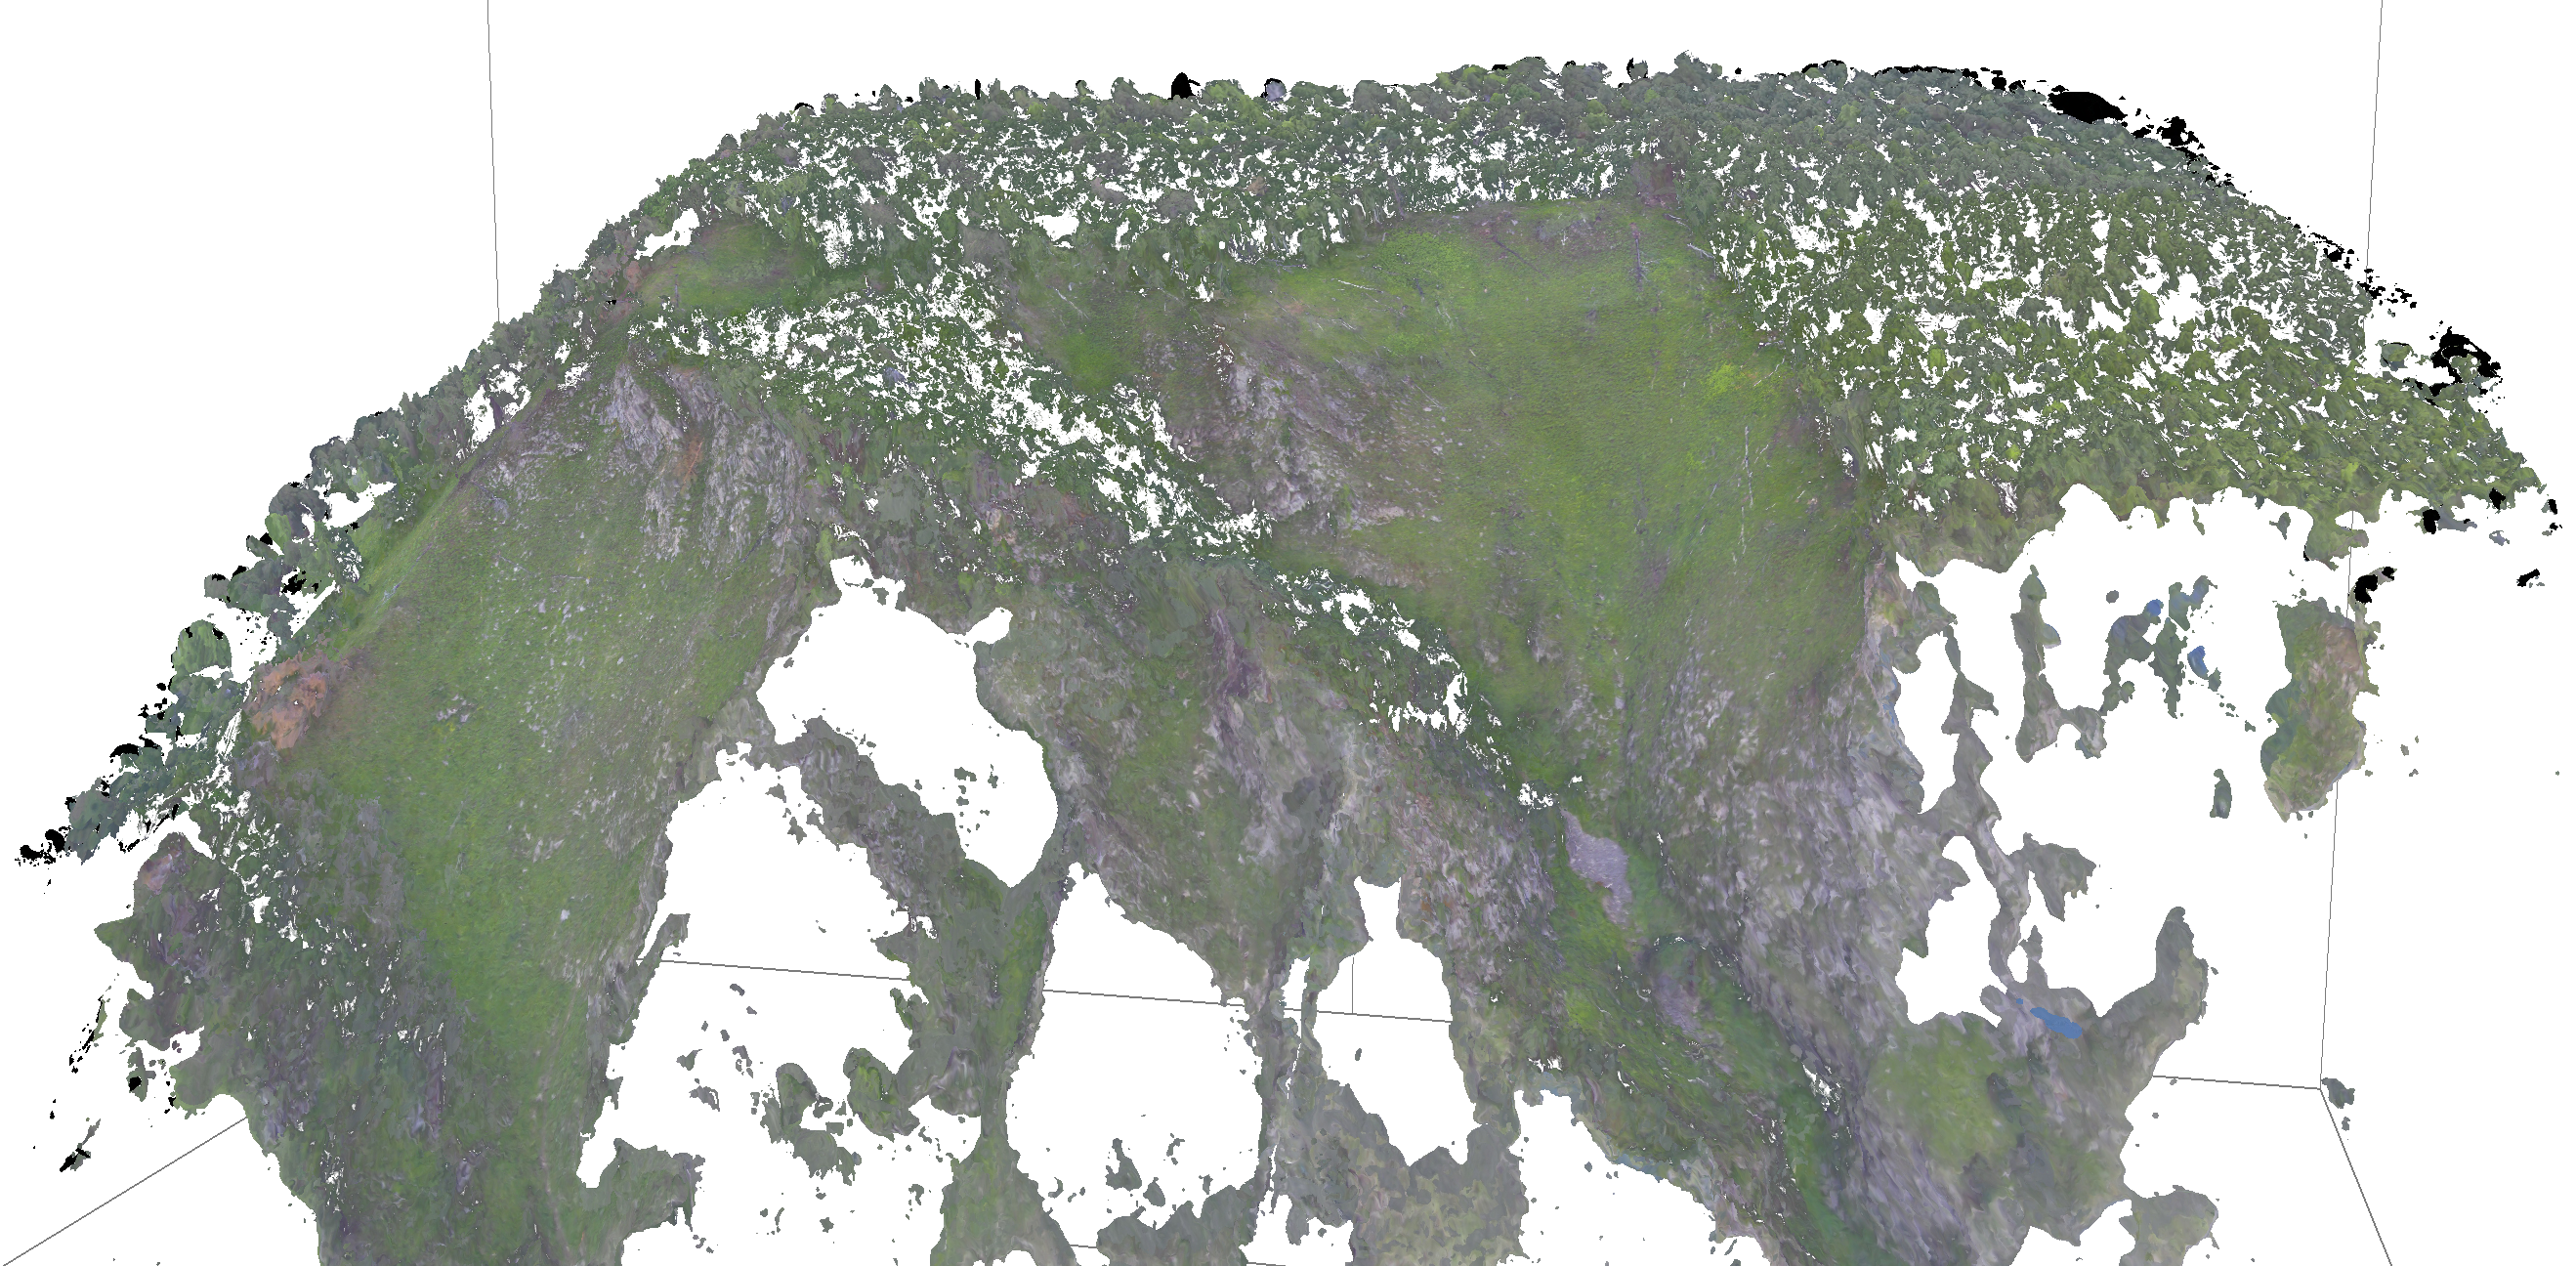
\includegraphics[width=0.9\textwidth]{authors/efremov-fig1.png}
  \end{center}
  \caption{Тайловая модель при выполнении съёмки с углом наклона камеры 90\dg}
  \label{fig:efremov-fig1}
\end{figure}


\item Съёмка по~методике, аналогичной моделированию зданий, включающая комбинирование наземных и~аэрофотограмметрических работ с~различными углами наклона камер слишком трудоёмка для мониторинга большого количества объектов площадью как~минимум по~нескольку квадратных километров.
\item Необходимо подбирать оптимальные по~соотношению <<качество результата/экономика работ>> модели фотокамер, в~том числе и~оборудования, с~режимом съёмки в~мульти\-спектральном спектре, с~учётом желательной минимизации массы и~стоимости владения комплексом, высокой точности и~детальности реконструкции местности, возможности работы при отрицательных температурах, достижения времени полёта не менее 1~ч.
\item Выбор наиболее подходящего программного обеспечения для обработки и~анализа материалов съёмки, как проприетарного, так и~бесплатного, для сравнительной характеристики и~предоставления результата специалистам ООО <<РЖД>>.
\item Создание компактного комплекса для возможности выполнения работы партией из~двух человек и~минимальным временем на~развёртку.

\end{enumerate}
\vspace{-8pt}

\textbf{Применяемое оборудование}

При выполнении поставленной задачи было использовано следующее оборудование:

\begin{itemize}[noitemsep]\vspace{-8pt}
\item тяжёлый гексакоптер SibGIS UAS (Unmanned Aerial System) (рис.~2);
\item двухосевые и~трехосевые гиростабилизированные подвесы лёгкого и~среднего классов.
\end{itemize}
\vspace{-8pt}

\begin{figure}[h!]
  \begin{center}
    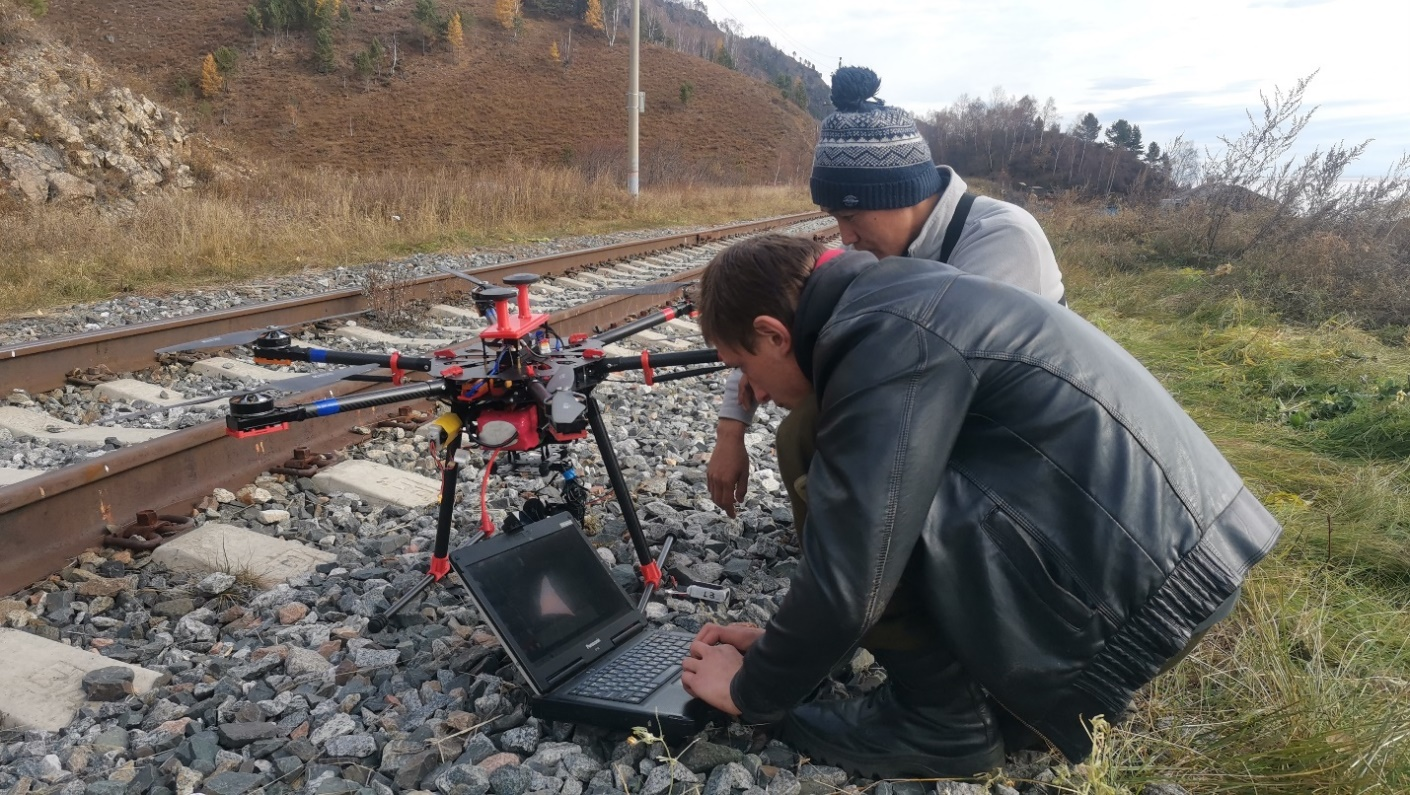
\includegraphics[width=0.9\textwidth]{authors/efremov-fig2.jpg}
  \end{center}
  \caption{Настройка комплекса на КБЖД}
  \label{fig:efremov-fig2}
\end{figure}


Камеры:

\begin{itemize}[noitemsep]\vspace{-8pt}
\item специализированные лёгкие камеры для аэрофотосъёмки Mapir Survey 2 и~3;
\item не специализированные, но подходящие для аэрофотосъёмки модели лёгких защищённых экшен-камер и~компактных цифровых фотокамер, таких как Sony RX0 и~GitUp Git3D;
\item B2B-фотокамеры семейства Sony QX/UMC.
\end{itemize}
\vspace{-8pt}

\textbf{Методика выполнения работ}

Для сбора необходимых нам данных было выполнено три серии опытно-методических съёмок на~опытном участке КБЖД, характеризующимся сложным рельефа, сопоставимым с~рельефом на~всей протяжённости железной дороги. Во всех трёх сериях использовался тяжёлый гексакоптер SibGIS UAS, который может переносить самые тяжёлые камеры и~подвесы, в~дальнейшем съёмку планируется проводить с~помощью более лёгкого БПЛА. Первые съёмки производились по~отработанной методике создания ЦМР, которую наш коллектив применяет в~геологической практике, а последующие работы были направлены на~оптимизацию технологии для данных условий.

После прибытия команды на~точку, откуда совершались полёты, производится развёртка оборудования: гексакоптер приводится в~рабочее положение, устанавливается базовая станция дифференциальной геодезической системы, применение которой необходимо для~создания точно привязанных центров фотографирования. Поскольку съёмка велась в~безреперном варианте, то <<базе>> дифференциальной станции требуется время на~позиционирование, для усреднения и~точной фиксации своего местоположения, после чего она будет передавать поправки на~ровер (в нашем случае в~качестве ровера выступает компьютер-компаньон полётного контроллера гексакоптера и~используются его GNSS-антенны) в~реальном времени. Выбор между внесением поправок при постобработке и~съёмки в~режиме кинематики реального времени~--- RTK сделан в~пользу последней, поскольку в~рамках данного класса задач размеры исследуемых участков не превышают первых десятков квадратных километров и~радиосвязь между базой и~ровером не теряется, а обработка требует меньших временных затрат.

Подвесы с~закреплёнными на~них камерами приводятся в~положение под необходимым углом.
\clearpage
С помощью специального модуля SibGIS Flight Planner (Паршин и~Морозов, 2017) [1] формируются полётные миссии, представляющие собой массив точек <<долгота~-- широта~-- высота>>, находящихся на~постоянной высоте над рельефом. Необходимая для этого цифровая модель рельефа создана заранее на~основе спутниковых данных Intermap Nextmap. Участок работ характеризуется перепадом высот в~несколько сотен метров, выполнять в~таких условиях фотосъёмку с~одного уровня или даже с~грубым обтеканием рельефа недопустимо, это приведёт к сложностям и~потере качества при обработке. Съёмка выполняется по~сети параллельных маршрутов, в~обычном случае скорость, высота и~продольное перекрытие между кадрами съёмки составляет 70--80\,\%, поперечное~--- 60--70\,\%. Съёмка велась на~высоте 125~м ($\sim$3--5~см/пиксель в~зависимости от применяемой камеры).

После проведения полевых работ выполняется обработка полученных данных съёмки. Если камера или её компьютер-компаньон не оснащены собственным GNSS-приёмником, перед каждым полётом производится синхронизация часов камеры с~точным временем.

На заключительном этапе выполняется фотограмметрическая обработка данных съёмки для получения 3D-моделей и~ортофотоплана.

Первая серия ОМР производилась со~съёмкой в~надир, затем были апробированы различные углы камеры: 45, 60 и~90\dg, с~обработкой вместе и~по отдельности, в~различных комбинациях (рис.~3).

\begin{figure}[h!]
  \begin{center}
    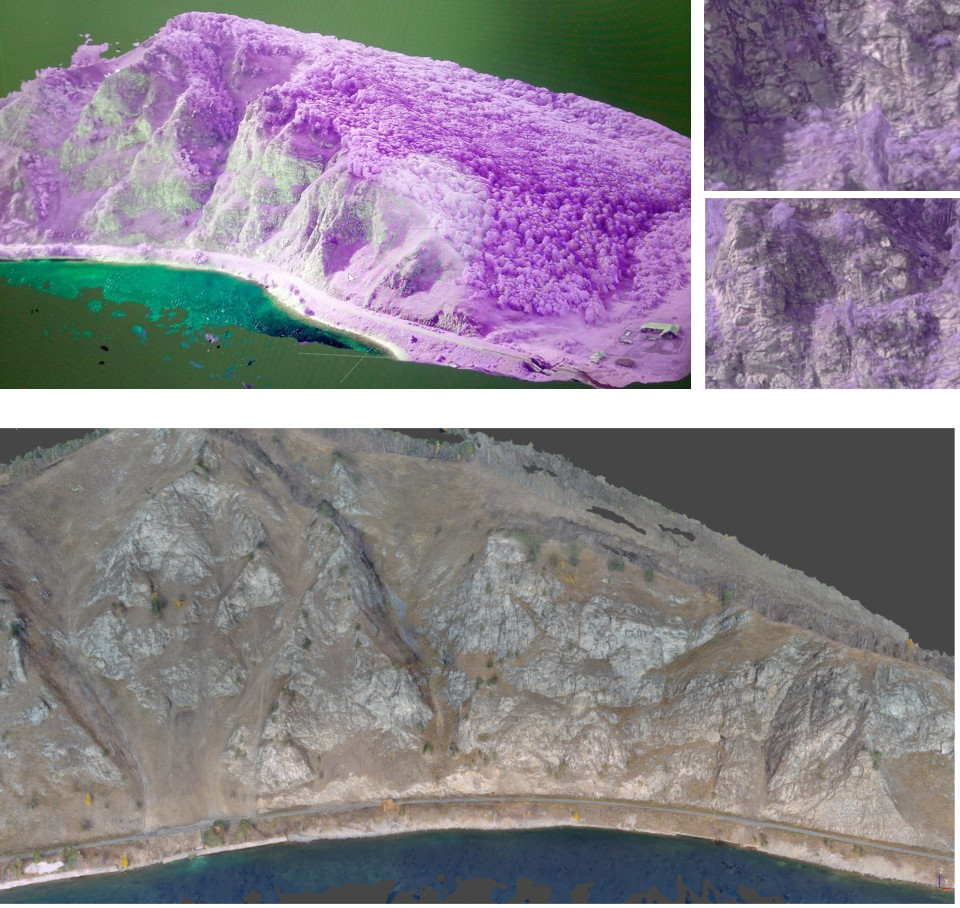
\includegraphics[width=0.9\textwidth]{authors/efremov-fig3.jpg}
  \end{center}
  \caption{Тайловая модель, построенная по результатам съёмки с углами наклона камеры 45 и 90 градусов: сверху~--- инфракрасный канал и крупные фрагменты модели; снизу~--- видимый диапазон)}
  \label{fig:efremov-fig3}
\end{figure}

\clearpage
\textbf{Выводы}

В результате проведённых исследований сделаны следующие заключения:
\begin{enumerate}[noitemsep]\vspace{-8pt}
\item Для получения полного объёма данных для построения детальной 3D модели достаточно производить съёмку с~двух углов наклона камеры~--- 45 и~90\dg (в надир).
\item При обработке фотографий следует заменять координаты в~метаданных фотоснимков с~камеры (если на~таковой установлен GPS модуль) на~координаты, взятые с~контроллера полётов, на~основе единства точного времени, записанного камерой и~ровером, поскольку для определения координат ровера используется дифференциальная станция, с~более точным определением местоположения.
\item Применение мультиспектральной камеры весьма желательно, поскольку позволяет более контрастно выделять трещины и~разломы на~тайловой модели. В перспективе это~создаст предпосылки для автоматизации дешифрирования опасных обстановок.
\item Использование трёхосевого подвеса, в~отличие от двухосевого, позволяет фиксировать камеру во всех трёх положениях, что даёт большую устойчивость, а при съёмке с~наклоном камеры не приходится менять настройки полёта, чтобы гексакоптер не~разворачивался при переходе на~соседний профиль.
\item Мониторинг склонов КБЖД с~использованием аэрофотограмметрии даёт более полное представление о состоянии массива, чем пеший обзор местности.
\item Применяемый метод и~оборудование возможно использовать не только на~участках КБЖД, но и~на других участках со~схожей проблематикой и~рельефом.
\end{enumerate}
\vspace{-8pt}

\begin{thebibliography}{99}

\bibitem{}\BibAuthor{Паршин А.~В., Морозов В.~А.} Навигационный модуль <<SibGIS Flight Planner>> // Свидетельство о регистрации программы для ЭВМ RU~2017615422, 16.05.2017.~--- Заявка №~2017612307 от 21.03.2017.
\bibitem{}\BibAuthor{Ahokas~J., Le Guern~P. Slettemeas~T., Syrdalen~E. et al.} Case-Study of Using Unmanned Aerial Vehicles for a Better Characterization of the Barents Sea Subsurface // First EAGE Workshop on Unmanned Aerial Vehicles.~--- Toulouse, 2019.~--- DOI:~10.3997/2214-4609.201903328.
\bibitem{}\BibAuthor{Bubniak I. M., Bubniak A. M., Gavrilenko O. D., Nikulishyn V. I., Golubinka I. I.}. Using laser scanning and digital photogrammetry for creation of virtual geological outcrops: case studies from the west of Ukraine // 18th International Conference on Geoinformatics~--- Theoretical and Applied Aspects. May 13--16, 2019. Kiev, Ukraine.~--- Kiev, 2019.~--- DOI: 10.3997/2214-4609.201902078.
\bibitem{}Geological models using digital outcrops from photogrammetry.~--- URL: https://www.georeka.com/geological\--models\--using\--digital\--outcrops\--from\--photogrammetry (ref. date: 26.10.2020).
\bibitem{}\BibAuthor{Parshin A.~V., Budyak A.~E., Babyak V.~N.} Interpretation of Integrated Aerial Geophysical Surveys by Unmanned Aerial Vehicles in Mining: a Case of Additional Flank Exploration // IOP Conf. Ser.: Earth Environ. Sci. 459 052079.~--- 2020.~--- DOI:~10.1088/1755-1315/459/5/052079.
\bibitem{}\BibAuthor{Parshin~A., Budyak~A., Chebokchinov~I., Sapunov~V., Bulnayev~A., Morozov~V.} Complex UAS-Geophysical Surveys at the First Stages of Geological Prospecting: Case in the Western Sayan (Russia) // First EAGE Workshop on Unmanned Aerial Vehicles.~--- Toulouse, 2019.~--- DOI:~10.3997/2214-4609.201903321.
\bibitem{}\BibAuthor{Rocca R}. Enhancing and Sharing Drone 3D Models with Geological Interpretation Using Move, Blender and Sketchfab Software // First EAGE Workshop on Unmanned Aerial Vehicles, Dec. 2019.~--- Toulouse, 2019.~--- DOI: 10.3997/2214-4609.201903331.
\end{thebibliography}
